\documentclass[12pt, letterpaper]{article}
\usepackage[utf8]{inputenc}
\usepackage[a4paper, total={7in, 10in}]{geometry}
\usepackage{amsmath}
\usepackage{tikz}
\usepackage{pgfplots}
\usepackage{setspace}
\usepackage{graphicx}
\graphicspath{ {./plots/} }

\title{STA222 Project}
\author{Ben Lirio}
\date{April 2}
\renewcommand{\baselinestretch}{1.5}

\begin{document}
\maketitle
\textit{I pledge my honor that I have abided by the Stevens Honor System}
\newpage
\section{}
Consider the provided sample Height and Weight of 200 individuals.
\subsection{}
Draw the empirical distribution functions of the height and the weight.
\[
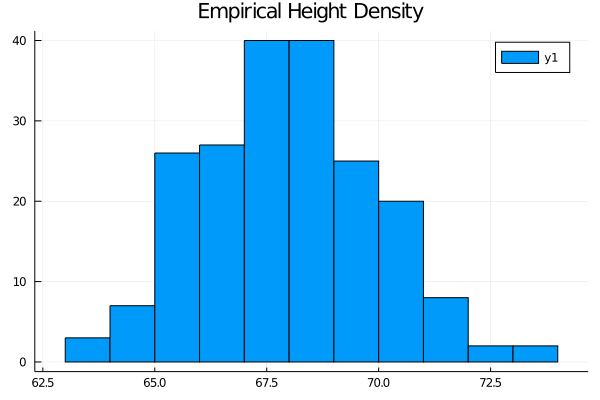
\includegraphics[scale=.5]{height_density.png}
\]
\[
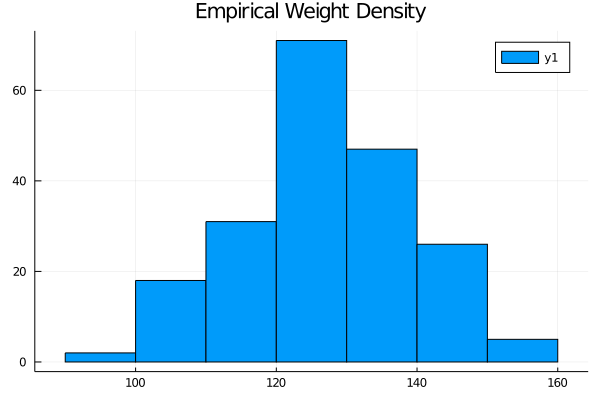
\includegraphics[scale=.5]{weight_density.png}
\]
\[
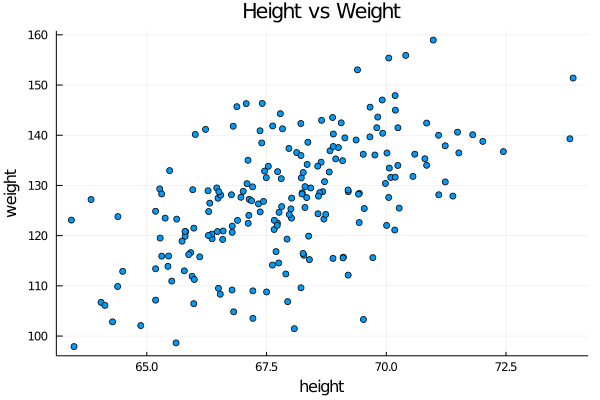
\includegraphics[scale=.5]{height_vs_weight.png}
\]
\subsection{}
Estimate the expected value, the median, and the variance of the height and the weight.
\newline
Let the random variable $X$ denote the real height distribution,
and let ${X_1, X_2, ..., X_{200}}$ represent the sample height provided.
\newline
Then an unbiased estimator of $E(X) = \mu$ is as follows
\[
\hat{\mu}_H = \frac{1}{200}\sum_{k=0}^{200} X_k = 67.95
\]
\begin{verbatim}
Julia 1.5.3
total = 0
for height in data.height
    total += height
end
n = length(data.height)
mean = total/n
\end{verbatim}
The variance can be calculated with
\[
\hat{\sigma}^2_H = \frac{1}{200}\sum_{k=0}^{200} (X_k-\hat{\mu})^2 = 3.747168
\]
\begin{verbatim}
Julia 1.5.3
total = 0
for height in data.height
    total += (height-mean)^2
end
n = length(data.height)
std = total/n
\end{verbatim}
The median  is
\[
\textrm{median}_H = 67.9280867
\]
\begin{verbatim}
sorted_height = sort(data.height)
mid_idx = Int(length(data.height)/2)
median = sorted_height[mid_idx]
\end{verbatim}
Using the exact same methods I can compute values for $W$
\[
\begin{split}
\hat{\mu}_W = 127.2223766 \\
\hat{\sigma}^2_W = 142.349941 \\
\textrm{media}_W = 127.869 \\
\end{split}
\]
\subsection{}
Construct a confidence interval for the expected values and the variances estimated in b.
\\
Using a confidence interval of $95\%$, $\alpha = 0.05$ and $Z_{\alpha / 2} = 1.69$
\\
With $95\%$ the following paramters have values in the range of
\[
\begin{split}
\mu_H \\
&= \bigg(\hat{\mu}_H - Z_{\alpha / 2}\cdot \frac{\sigma_H}{\sqrt{n}},
\hat{\mu}_H + Z_{\alpha / 2}\cdot \frac{\sigma_H}{\sqrt{n}}\bigg) \\
&= \bigg(67.95 - \frac{\sqrt{3.747168}}{\sqrt{200}}, 67.95 + \frac{\sqrt{3.747168}}{\sqrt{200}}\bigg) \\
&= (67.6762, 68.2238) \\
\mu_W \\
&= \bigg(\hat{\mu}_W - Z_{\alpha / 2}\cdot \frac{\sigma_W}{\sqrt{n}},
\hat{\mu}_W + Z_{\alpha / 2}\cdot \frac{\sigma_W}{\sqrt{n}}\bigg) \\
&= \bigg(127.22237 - \frac{\sqrt{142.35}}{\sqrt{200}}, 127.22237 + \frac{\sqrt{142.35}}{\sqrt{200}}\bigg) \\
&= (126.379, 128.066) \\
\end{split}
\]

\subsection{}
Estimate the height of the tallest 10\% of the people.
\\
I will estimate the population distribution Guassian distribution with 
$\mu = 67.95$ and $\sigma = 1.93576$
\[
\begin{split}
Z = invNorm(0.9) = 1.28155 \\
height \ge \mu + Z \cdot \sigma = 70.4308
\end{split}
\]
The top $10\%$ of people are taller than $70.4308$ in

\subsection{}
Estimate the proportion of pople taller than 70.5 inches. Does the data support the 
claim that 10\% of the population is taller than 70.5 inches? Calculate and interpret the
p-value of the statistics.
\\
The $Z$-value is
\[
\frac{70.5 - \mu}{\sigma} = \frac{70.5-67.95}{1.93576} = 1.31731
\]
Using this for an I can calulate the p-value
\[
\textrm{normCdf}(-\infty, 1.31731, \mu = 0, \sigma=1) = 0.906133
\]
No does evidence does not support this. Instead it supports that only 
$100\cdot(1 - 0.906133)\% = 9.38674\%$ of the population is over $70.5$ in
\subsection{}
Estimate the proportion of pople heavier than 125 lb. At level of significance 0.9, test the
hypothesis that less than half of the population weigh more than 125 lb?
\\
First calculate the $Z$ value
\[
\frac{125-\mu}{\sigma} = \frac{125-127.22237}{11.9311} = -0.186267
\]
Then I can use this value to test find the estimated proportion
\[
\textrm{normCdf}(-0.86267, \infty, \mu=0, \sigma=1) = 0.805841
\]
Approximatly $80.5841\%$ of the population is over $125$ lb
\\
The null hypothesis is that $\mu > 125$
\\
I fail to reject the null becuase my significance of $0.9$ is greater than $0.805841$
\newpage
\section{Problem}
let $g: [0,1]^n \rightarrow R$ be a continuous function of $n$ variables, defined over the $n$-dimensional
unit cube $C = [0, 1]^n$. One way to calculate the integral
\[
I = \int_{0}^{1} ... \int_{0}^{1} g(x_1, ..., x_n) dx_1 ... dx_n
\]
is known as the Monte Carlo technique, which consists in the following.
Assume that $X_i, i = 1, ... n$, are independent random variable with the
uniform distribution on the interval $[0, 1]$. This implies that for any nice
subset of $A$ of the unit cube $C$ the probability $P{(X_1,..., X_n) \in A}$ is
equal to the "volume" of $A$. We preform a large number of the following experiment.
Observe values $x_1, ..., x_n$ of the random variables and evaluate the function $g(x_1, ..., x_n)$.
We use the results to evaluate the integral $I$.
\subsection{}
Express the integral $\textbf{I}$ is the expected value of $g(X_1, ..., X_n)$.
\\
The expected value is
\[
\textbf{I} = \int_{0}^{1}x_1\int_{0}^{1}x_2 \int_{0}^{1}x_ng(x_1, x_2, ..., x_n)\ dx_1,...,dx_n
\]
Now since $X_1, X_2, ..., X_n$ are all independent
\[
g(x_1, x_2,...,x_n) = g(x_1)g(x_2)...g(x_n)
\]
I can then substitute that into the integral
\[
\textbf{I} = \int_{0}^{1}x_1\int_{0}^{1}x_2 \int_{0}^{1}x_ng(x_1)g(x_2)...g(x_n)\ dx_1,...,dx_n
\]
I can then move the $g(x_i)$ left as far as the integrals allow
\[
\textbf{I} = \int_{0}^{1}x_1g(x_1)\int_{0}^{1}x_2g(x_2) \int_{0}^{1}x_ng(x_n)\ dx_1,...,dx_n
\]
This is equivalent to
\[
\mu_{X_1}\cdot \mu_{X_2}\cdot ... \cdot \mu_{X_n}
\]
Since $X_1, X_2, ..., X_n$ are all uniform $[0, 1]$ with $\mu = 0.5$, then the expected value is
\[
(0.5)^n
\]
\subsection{}
What statistical estimator will provide an estimate for $\textbf{I}$?
\\
The statistical estimator for $\textbf{I}$, is $\hat{\mu}_G$
\subsection{}
Use \underline{this technique} to evaluate the following integral:
\[
	\int_{0}^{1} \int_{0}^{1} |sin(min{x,|x-y^2|})|e^{-xy} dxxdy
\]

Here $|a|$ is the absolute value of the number a, and $min{a, b}$ is a function
that equals to the smaller of the two. (Direct integral evalucation using some
software is not acceptable.)
You may use any software for you calculations. Provide printout.
\\
Here is the printout of the MonteCarlo simulation
\\
To create this I rounded the $(x, y)$ cordinates to the nearest $100^{th}$.
For the speckles I could can have three options to remove them. (1) run more samples.
(2) Make a bigger coordinate estimate. (3) Interpolate between near points.\\
Instead I will leave them in becuase it shows that the monte carlo method is approximate
\\
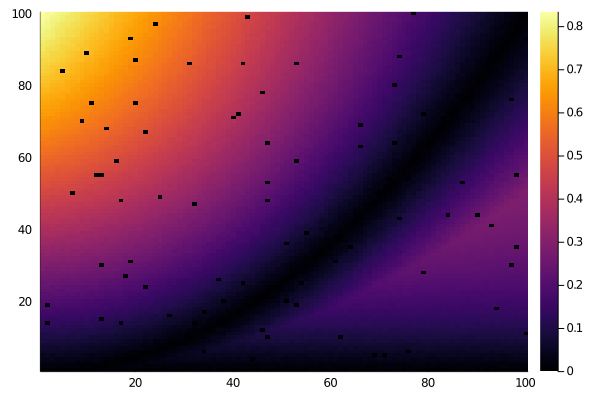
\includegraphics[scale=.5]{heatmap.png}
\\
By taking a sum of the pdf values I get \textbf{0.246707}
\\
I went low level for the coding and implemented my own
\begin{itemize}
	\item random number generator
	\item sin() approximation
	\item natural exponent approximation
	\item and csv marsheller
\end{itemize}

\begin{verbatim}
#include <stdlib.h>
#include <stdbool.h>
#include <unistd.h>
#include <time.h>
#include <stdio.h>
#include <string.h>
#include <errno.h>
#include <fcntl.h>

#define NORMALIZE(X) (X)/(float)(unsigned int)(~0)
#define MIN(X, Y) (X) < (Y) ? (X) : (Y)
#define PI 3.1415926535897932384626433832795028841972
#define E 2.7182818284590452353602874713526624977572
#define BUFSIZE 124

typedef struct rand_state_t {
    unsigned int a;
    unsigned int c;
    unsigned int cur;
    unsigned int start;
} rand_state_t;

rand_state_t new_rand_state(unsigned int seed) {
    rand_state_t rand_state;
    rand_state.a = 1664525;
    rand_state.c = 1013904223;
    rand_state.cur = seed;
    rand_state.start = seed;
    return rand_state;
}

unsigned int uniform_rand(rand_state_t* s) {
    s->cur = s->a * s->cur + s->c;
    return s->cur;
}

float small_sin_approx(float x) {
    if (x > 1) {
        fprintf(stderr, "Error: This function is only for values less than or equal to 1\n");
        exit(EXIT_FAILURE);
    }
    int degree = 5;
    float coeff[] = {
        0.007252,
        0.001613,
        -0.167616,
        0.000244,
        0.999978,
        0
    };
    float sum = 0;
    for (int i = 0; i <= degree; i++) {
        float poly = 1;
        for (int j = degree; j > i; j--) {
            poly *= x;
        }
        sum += coeff[i]*poly;
    }
    return sum;
}

float small_neg_natural_exp_approx(float power) {
    if (power < -1.0 || power > 0.0) {
        fprintf(stderr, "Error: Expected power to be in range [-1, 0]\n");
    }

    int degree = 5;
    float coeff[] = {
        -0.217251596861,
        -0.406386432184,
        -0.146323730534,
        0.410655519563,
        0.9914267988415,
        1
    };
    float sum = 0;
    for (int i = 0; i <= degree; i++) {
        float poly = 1.0;
        for (int j = degree; j > i; j--) {
            poly *= power;
        }
        sum += coeff[i]*poly;
    }
    return sum;
}

float pdf(float x, float y) {
    float exp = small_neg_natural_exp_approx(-x*y);
    float min_term_2 = x-y*y < 0 ? -(x-y*y) : (x-y*y);
    float sin_term = MIN(x, min_term_2);
    // sin will always be positive so no need to abs()
    return small_sin_approx(sin_term)*exp;
}

int main() {
    int seed = time(NULL);
    rand_state_t rand_state = new_rand_state(seed);
    unsigned int rand_bits;
    float x;
    float y;
    int sample_size = 50000;
    float** data = malloc(sizeof(float*)*sample_size);
    for (int i = 0; i < sample_size; i++) {
        data[i] = malloc(sizeof(float)*3); // Tuple (x, y, pdf(x, y))
    }
    for (int i = 0; i < sample_size; i++) {
        rand_bits = uniform_rand(&rand_state);
        x = NORMALIZE(rand_bits);
        rand_bits = uniform_rand(&rand_state);
        y = NORMALIZE(rand_bits);
        data[i][0] = x;
        data[i][1] = y;
        data[i][2] = pdf(x, y);
    }
    int fd;
    if ((fd = open("data.csv", O_CREAT|O_RDWR, 0644)) == -1) {
        fprintf(stderr, "Error: failed to create or open 'data.csv'. %s.\n", strerror(errno));
        return EXIT_FAILURE;
    }
    char buf[BUFSIZE];
    ssize_t n;
    char* header = "x,y,pdf\n";
    n = write(fd, header, strlen(header));
    if (n != strlen(header)) {
        fprintf(stderr, "Error: Failed to print %lu bytes. %s.\n", strlen(header), strerror(errno));
        return EXIT_FAILURE;
    }
    
    for (int i = 0; i < sample_size; i++) {
        sprintf(buf, "%f,%f,%f\n",data[i][0], data[i][1], data[i][2]);
        n = write(fd, buf, strlen(buf));
        if (n != strlen(buf)) {
            fprintf(stderr, "Error: Failed to print %lu bytes. %s.\n", strlen(buf), strerror(errno));
            return EXIT_FAILURE;
        }
    }

    if (close(fd) != 0) {
        fprintf(stderr, "Error: failed to close 'data.csv'. %s.\n", strerror(errno));
        return EXIT_FAILURE;
    }
    for (int i = 0; i < sample_size; i++) {
        free(data[i]);
    }
    free(data);
}
\end{verbatim}

\end{document}
